\chapter{Special Relativity: Frames, Simultaneity, and the Lorentz Transformation}

These notes follow Leonard Susskind's lecture, with curation for this edition by LazyingArt LLC. The lecture opens by setting the agenda for the quarter: first special relativity done carefully as kinematics, then relativistic dynamics, and only later a more conceptual pass through general relativity. We therefore begin where the lecture itself begins in earnest, with the meaning of a frame of reference, with clocks and meter sticks, and with the insistence that the right way to start a relativity problem is to draw spacetime.

\section{A Short Framing Note}

Relativity, in the sense used here, is the statement that the laws of physics should not depend on the uniform motion of the observer. That idea is older than Einstein. Susskind likes to make the point with a train moving so smoothly that nothing inside it rattles or shakes. In such a train, the laws of juggling are the same as they are in a train standing at the station. If we throw a ball upward, we do not have to compensate for the train's motion in order to catch it again. The physics inside the smoothly moving train is the same physics.

What Einstein changes is not the relativity principle itself, but the structure of space and time needed to preserve it once light is brought into the story. Newton imagined a universal time, almost a God's time, common to all clocks everywhere. Einstein keeps the relativity principle and abandons the universality of simultaneity. The lecture proceeds exactly in that order: first Galileo, then the crisis created by light, then the reconstruction of space and time.

\section{Reference Frames as Lattices of Meter Sticks and Clocks}

\begin{definition}
A reference frame is an imaginary lattice of meter sticks filling space, with a clock at each lattice point. An event is a point in spacetime labeled by a spatial location in that lattice and by the reading of the appropriate clock.
\end{definition}

The lecture immediately turns this operational definition into a picture. Time is drawn vertically, space horizontally, and for the moment we suppress the \(y\) and \(z\) directions and work only with one spatial coordinate \(x\). Every point on the board then represents a place together with a time.

The horizontal axis is the set of events with \(t=0\). The vertical line through the origin is the worldline of the point \(x=0\). The next vertical line is the worldline of the point \(x=1\), then \(x=2\), and so on. As the clocks tick upward in time, the meter-stick lattice produces a family of constant-position worldlines. When we add horizontal lines of constant time, the whole picture becomes a spacetime lattice.

\begin{figure}
\centering

\includegraphics[width=0.62\textwidth]{lecture_01_figure_02.png}
\caption{Rest-frame time axis and the emerging spacetime lattice.}
\end{figure}

\begin{figure}
\centering
\begin{tikzpicture}[scale=0.95]
\draw[->] (-1.2,0) -- (5.2,0) node[right] {$x$};
\draw[->] (0,-0.2) -- (0,4.8) node[above] {$t$};
\foreach \x in {-1,1,2,3,4}
  \draw[gray] (\x,0) -- (\x,4.4);
\foreach \y in {1,2,3,4}
  \draw[gray] (-1.0,\y) -- (4.4,\y);
\fill (0,0) circle (1.5pt);
\node[below left] at (0,0) {$0$};
\node[left] at (0,1) {$1$};
\node[left] at (0,2) {$2$};
\node[left] at (0,3) {$3$};
\node[below] at (1,0) {$1$};
\node[below] at (2,0) {$2$};
\node[below] at (3,0) {$3$};
\end{tikzpicture}
\caption{A clean reconstruction of the stationary spacetime lattice: constant-position worldlines are vertical and constant-time slices are horizontal.}
\end{figure}

The board at this point is still sparse, and that is important. Susskind is not yet racing toward formulas. He is teaching us how to think about a frame: as a grid of locations and synchronized clocks, made visible in spacetime before any transformation law is written down.

\section{Galilean Relativity from the Spacetime Picture}

The lecture now brings back the train picture and makes it geometrical. Let the stationary observer use coordinates \((x,t)\), and let the moving observer ride in a train whose origin moves with constant velocity \(v\). In the stationary frame the moving origin has the worldline
\begin{equation}
x=vt.
\end{equation}
The next point of the moving lattice traces a parallel line shifted by a fixed amount, then the next one, and so on. In a spacetime plot the moving family of constant-position lines is tilted.

That tilt is the whole content of Galilean kinematics. An event with stationary coordinates \((x,t)\) has, for the moving observer, the same time but a different spatial coordinate, because the moving origin has shifted by the amount \(vt\). Reading directly from the diagram, one arrives at
\begin{align}
t' &= t, \\
x' &= x-vt.
\end{align}
Susskind is careful about the order here. He does not begin from algebra and then draw a picture afterward. He draws the picture and then reads the equations off the board.

\begin{figure}
\centering

\includegraphics[width=0.72\textwidth]{lecture_01_figure_03.png}
\caption{Galilean coordinate shift beside the spacetime sketch.}
\end{figure}

\begin{figure}
\centering
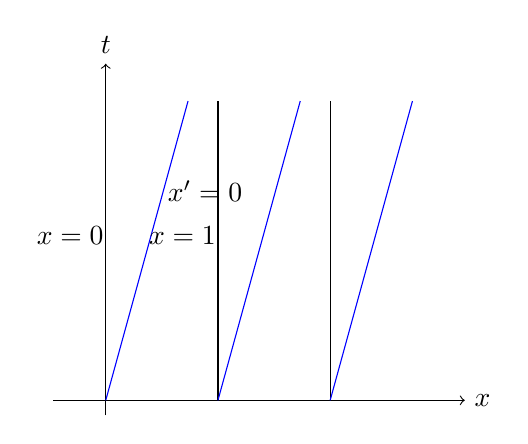
\begin{tikzpicture}[scale=0.95]
\draw[->] (-0.7,0) -- (4.8,0) node[right] {$x$};
\draw[->] (0,-0.2) -- (0,4.5) node[above] {$t$};

\draw[black] (0,0) -- (0,4.0);
\draw[black] (1.5,0) -- (1.5,4.0);
\draw[black] (3.0,0) -- (3.0,4.0);

\draw[blue] (0,0) -- (1.1,4.0);
\draw[blue] (1.5,0) -- (2.6,4.0);
\draw[blue] (3.0,0) -- (4.1,4.0);

\node[left] at (0.1,2.2) {$x=0$};
\node[left] at (1.6,2.2) {$x=1$};
\node[right] at (0.7,2.8) {$x'=0$};
\end{tikzpicture}
\caption{Stationary worldlines and the tilted moving family from which the Galilean shift is read.}
\end{figure}

We can invert the relation as well. Since \(t=t'\), the inverse form is
\begin{align}
t &= t', \\
x &= x'+vt'.
\end{align}
The lower inverse equation is cropped in the board frame, and Susskind briefly phrases it as \(x=x'+vt\). But because \(t=t'\) in Galilean relativity, the intended inverse equation is the canonical one just written.

This is also the point in the lecture where the train analogy and the mathematics meet cleanly. The first pair of equations tells the stationary observer how to convert his description into the moving observer's description; the second pair tells us how to go back. Galilean relativity is, in that sense, a theory of transformations between frames.

\section{What Galileo Gets Right}

Susskind now pauses and asks the right question: what is invariant? He does not want the transformation law to float free of physics.

Take two events at the same time \(t\), with positions \(x_1\) and \(x_2\). In the moving frame,
\begin{align}
x_1' &= x_1-vt, \\
x_2' &= x_2-vt.
\end{align}
Subtracting the two,
\begin{equation}
x_2'-x_1'=(x_2-vt)-(x_1-vt)=x_2-x_1.
\end{equation}
So the spatial separation of two simultaneous events is invariant under Galilean transformations. The individual coordinates are not invariant, but their difference is.

At this stage the lecture also raises a natural worry. How do we know that time really remains universal when a clock is carried around? Galileo himself did not know in any strict modern sense. It was, as Susskind says, frankly a guess, though a very good one. For ordinary clocks moved around at ordinary speeds, the agreement is fantastically precise. Only at sufficiently high speeds does the guess fail, and that failure is exactly what special relativity is about.

Now let a particle follow a trajectory \(x(t)\). The moving observer sees
\begin{equation}
x'(t)=x(t)-vt.
\end{equation}
So position is not invariant. Different observers attach different spatial coordinates to the same particle. Differentiating once,
\begin{equation}
\frac{dx'}{dt}=\frac{dx}{dt}-v,
\end{equation}
and therefore velocity is not invariant either. This is obvious from ordinary experience: if I move along beside your arrow, I judge its speed differently from you.

Differentiate once more:
\begin{equation}
\frac{d^2x'}{dt^2}=\frac{d^2x}{dt^2},
\end{equation}
because the relative velocity \(v\) between inertial frames is constant. Acceleration is invariant.

This is the Newtonian payoff. If the force between two objects depends only on the distance between them, and if that distance is invariant, then the force is also invariant. If acceleration is invariant as well, then
\begin{equation}
F=ma
\end{equation}
has precisely the right structure to serve as a law of motion that all inertial observers can share, provided mass itself is invariant. In this sense Newton's laws are invariant under Galilean coordinate transformations.

The lecture's point is not merely historical courtesy. Galileo and Newton were not making a naive mistake. For mechanics at low velocities, the whole scheme is extraordinarily successful.

\section{Maxwell's Challenge and Einstein's Return to First Principles}

The next move is the crisis. Galilean relativity works beautifully for mechanics, but electromagnetism changes the stakes. Maxwell's equations predict a definite speed for light, and if Maxwell's equations are taken seriously as laws of nature, then the speed of light ought to be the same for every inertial observer.

Galilean kinematics says otherwise. If a light ray in the stationary frame satisfies
\begin{equation}
x=ct,
\end{equation}
then the moving observer would assign
\begin{equation}
x'=x-vt=(c-v)t.
\end{equation}
So under a Galilean transformation the moving observer sees light propagate at speed \(c-v\), not at \(c\). That is exactly what one would expect for sound waves or water waves. Indeed Susskind stresses that this was not a crazy expectation. It was the natural expectation.

The historical temptation, before Einstein, was to conclude that there must be a preferred frame, a kind of God's frame, in which Maxwell's equations are exactly right and in which light really travels at speed \(c\). Einstein's move is more radical and more economical. He keeps the relativity principle and forces space and time to adapt. In the lecture this comes in the form of two postulates:
\begin{enumerate}
\item The laws of physics are identical in every inertial frame.
\item The speed of light is the same in every inertial frame.
\end{enumerate}

But these postulates do not yet tell us how to assign coordinates. So Einstein goes back to first principles and asks what it means for clocks at different places to be synchronized. The answer is operational. Put an observer at the midpoint between two endpoint clocks. Emit flashes from the endpoints when the endpoint clocks read the same time. If the midpoint observer receives the flashes simultaneously, the clocks are synchronized.

This is the point where the lecture stops being Newtonian in spirit. If a second observer moves past that synchronized apparatus, the two flashes no longer arrive at the moving midpoint at the same instant. The moving observer must therefore conclude that the original emissions were not simultaneous. Simultaneity is not absolute.

\subsection{Question \& Answer}

\paragraph{Question.} Why not synchronize clocks with sound instead of light?

\paragraph{Answer.} One can synchronize clocks with sound in a frame in which the air is at rest. But then one immediately discovers that moving observers measure different sound speeds. Sound propagates in a medium, and motion relative to that medium matters. In an open-air train moving through still air, sound would be a bad messenger of relativity. Light is chosen for the opposite reason: Einstein's postulate is that light has the same speed for every inertial observer, so light is exactly the signal with which the notion of simultaneity must be rebuilt.

The lecture now asks its central quantitative question: if the stationary observer calls one pair of distant events simultaneous, which pair does the moving observer call simultaneous instead?

\section{The Geometry of Relativity of Simultaneity}

Susskind now slows down and makes the question geometric. He sets \(c=1\), so that space and time are measured in compatible units and light rays run at \(45^\circ\). A right-moving light ray has the form
\begin{equation}
x=t+d,
\end{equation}
and a left-moving light ray has the form
\begin{equation}
x=-t+d'.
\end{equation}
In particular, the light ray from the origin satisfies \(x=t\).

He then lays out the rest-frame synchronization experiment with endpoints separated by equal distances \(L\). The midpoint observer sits between them. Once the moving frame is added, the question becomes concrete: which event on the right-moving family is simultaneous, in the moving sense, with the event at the origin?

\begin{figure}
\centering

\includegraphics[width=0.72\textwidth]{lecture_01_figure_04.png}
\caption{Light-ray line \(x=t\) in the simultaneity construction.}
\end{figure}

On the board only the label \(x=t\) is clearly legible. The shifted moving worldlines are reconstructed from the transcript and from the geometry as
\begin{equation}
x=vt,\qquad x=vt+L,\qquad x=vt+2L.
\end{equation}
One transcript line later drops the factor of \(t\), but the construction itself makes the intended form unambiguous.

\begin{figure}
\centering
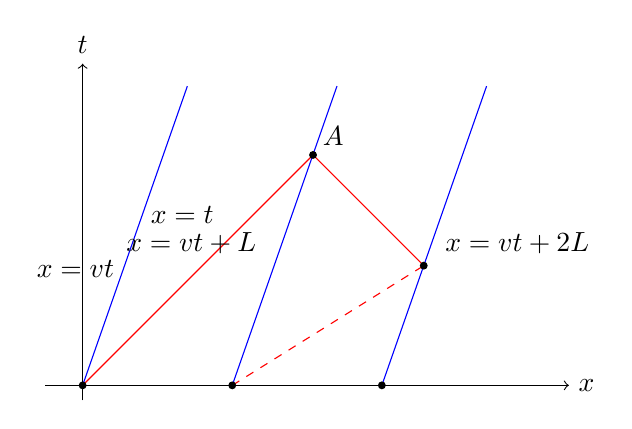
\begin{tikzpicture}[scale=0.95]
\draw[->] (-0.5,0) -- (6.5,0) node[right] {$x$};
\draw[->] (0,-0.2) -- (0,4.3) node[above] {$t$};

\draw[blue] (0,0) -- (1.4,4.0);
\draw[blue] (2.0,0) -- (3.4,4.0);
\draw[blue] (4.0,0) -- (5.4,4.0);

\draw[red] (0,0) -- (3.08,3.08);
\draw[red] (3.08,3.08) -- (4.56,1.60);
\draw[red,dashed] (2.0,0) -- (4.56,1.60);

\fill (0,0) circle (1.5pt);
\fill (2.0,0) circle (1.5pt);
\fill (4.0,0) circle (1.5pt);
\fill (3.08,3.08) circle (1.5pt);
\fill (4.56,1.60) circle (1.5pt);

\node[left] at (0.55,1.55) {$x=vt$};
\node[left] at (2.45,1.9) {$x=vt+L$};
\node[right] at (4.72,1.9) {$x=vt+2L$};
\node[left] at (1.88,2.28) {$x=t$};
\node[above right] at (3.08,3.08) {$A$};
\end{tikzpicture}
\caption{Reconstruction of the simultaneity argument. The screenshot preserves the board evidence; the redraw makes the equations explicit.}
\end{figure}

The lecture's rhythm at this point is exact: it first argues qualitatively that the two frames will disagree, and then asks, ``Can we do it quantitatively?'' The answer is yes.

\paragraph{Worked derivation.} Let \(A\) be the point where the forward light ray \(x=t\) meets the shifted worldline \(x=vt+L\). Then \(A\) is determined by
\begin{align}
x &= t, \\
x &= vt+L.
\end{align}
Substituting \(x=t\) into the second equation gives
\begin{equation}
t=vt+L,
\end{equation}
so
\begin{equation}
(1-v)t=L,
\end{equation}
and therefore
\begin{equation}
t_A=\frac{L}{1-v},\qquad x_A=\frac{L}{1-v}.
\end{equation}

Now follow a backward-going light ray from \(A\). A left-moving light ray has the form
\begin{equation}
x=-t+b,
\end{equation}
or equivalently
\begin{equation}
x+t=b.
\end{equation}
To determine \(b\), use the fact that the ray passes through \(A\). At \(A\), we have \(x=t=L/(1-v)\), so
\begin{equation}
b=x_A+t_A=\frac{2L}{1-v}.
\end{equation}
Thus the backward light ray is
\begin{equation}
x+t=\frac{2L}{1-v}.
\end{equation}

The event we want is where this backward light ray meets the next shifted worldline \(x=vt+2L\). So we solve
\begin{align}
x+t &= \frac{2L}{1-v}, \\
x &= vt+2L.
\end{align}
Substituting the second equation into the first yields
\begin{equation}
vt+2L+t=\frac{2L}{1-v}.
\end{equation}
Rearranging,
\begin{equation}
(1+v)t=2L\left(\frac{1}{1-v}-1\right)=2L\frac{v}{1-v},
\end{equation}
and therefore
\begin{equation}
t=\frac{2Lv}{1-v^2}.
\end{equation}
Putting this back into \(x=vt+2L\), we obtain
\begin{equation}
x=\frac{2L}{1-v^2}.
\end{equation}
What matters is not these coordinates by themselves, but their ratio:
\begin{equation}
\frac{t}{x}=v.
\end{equation}
So the moving observer's simultaneity line through the origin is
\begin{equation}
t=vx.
\end{equation}

This is the lecture's geometric payoff. The moving observer's time axis is
\begin{equation}
x=vt,
\end{equation}
because that is the worldline of the moving origin. The moving observer's line of simultaneity is
\begin{equation}
t=vx,
\end{equation}
because those are the points assigned the same moving time. The two are tilted symmetrically with respect to the light rays.

Restoring dimensions requires only one correction:
\begin{equation}
t=\frac{v}{c^2}x.
\end{equation}
This formula makes clear why simultaneity appears absolute in ordinary life. The denominator \(c^2\) is enormous. Only when velocities become appreciable compared with the speed of light does the tilt become visible.

\section{From Tilted Axes to the Lorentz Transformation}

The lecture now performs an instructive cleanup. It erases the clutter of the construction and keeps only what the construction has taught us: the unprimed axes, the primed axes, and the light rays. In units with \(c=1\), the picture has what Susskind calls a lovely symmetry.

\begin{figure}
\centering

\includegraphics[width=0.72\textwidth]{lecture_01_figure_05.png}
\caption{Symmetric \(c=1\) spacetime diagram.}
\end{figure}

\begin{figure}
\centering
\begin{tikzpicture}[scale=1.0]
\draw[->] (-2.2,0) -- (5.2,0) node[right] {$x$};
\draw[->] (0,-0.2) -- (0,4.9) node[above] {$t$};

\draw[red] (0,0) -- (3.9,3.9);
\draw[red] (0,0) -- (-1.8,1.8);

\draw[blue] (0,0) -- (1.8,4.5);
\draw[blue,dashed] (0,0) -- (4.5,1.8);

\node[right] at (3.9,3.9) {$x=t$};
\node[left] at (-1.8,1.8) {$x=-t$};
\node[above] at (1.8,4.5) {$x'=0$};
\node[right] at (4.5,1.8) {$t'=0$};
\end{tikzpicture}
\caption{Cleaned \(c=1\) diagram showing the primed time axis, the primed simultaneity axis, and the two light rays.}
\end{figure}

The lecture later shifts on the board to upper-case \(X,T\), but the substance is unchanged. We keep lower-case \(x,t\) throughout.

The geometry already tells us the zero-sets of the primed coordinates. Since the moving origin is the line \(x=vt\), the quantity \(x'\) must vanish there. That is the surviving content of Galileo's old formula \(x'=x-vt\): even if the exact coefficient changes, the zero-set must remain the same. This motivates
\begin{equation}
x'=\frac{x-vt}{F(v)}.
\end{equation}
Likewise, because the moving simultaneity axis is the line \(t=vx\), the quantity \(t'\) must vanish there. So we write
\begin{equation}
t'=\frac{t-vx}{G(v)}.
\end{equation}
Here \(F(v)\) and \(G(v)\) are unknown denominator functions. This matters: when the lecture later concludes that \(F(v)=\sqrt{1-v^2}\), it is the denominator that equals that square root.

Now use the invariance of light speed. A light ray satisfying \(x=t\) in the unprimed frame must satisfy \(x'=t'\) in the primed frame. Substituting \(x=t\) gives
\begin{align}
x' &= \frac{(1-v)t}{F(v)}, \\
t' &= \frac{(1-v)t}{G(v)}.
\end{align}
These must agree for every such light ray, so
\begin{equation}
F(v)=G(v).
\end{equation}
Hence
\begin{equation}
x'=\frac{x-vt}{F(v)},\qquad t'=\frac{t-vx}{F(v)}.
\end{equation}

We still do not know \(F(v)\). To determine it, multiply through:
\begin{align}
F(v)x' &= x-vt, \\
F(v)t' &= t-vx.
\end{align}
To solve for \(x\), multiply the second equation by \(v\) and add it to the first. The \(vt\) terms cancel:
\begin{equation}
(1-v^2)x=F(v)\bigl(x'+vt'\bigr),
\end{equation}
so
\begin{equation}
x=\frac{F(v)\bigl(x'+vt'\bigr)}{1-v^2}.
\end{equation}
By the same algebra,
\begin{equation}
t=\frac{F(v)\bigl(t'+vx'\bigr)}{1-v^2}.
\end{equation}

Now comes what Susskind calls the other half of the key. The forward and inverse transformations should have the same form, except that the sign of the relative velocity reverses. This reciprocity condition demands
\begin{equation}
\frac{F(v)}{1-v^2}=\frac{1}{F(v)}.
\end{equation}
Multiplying through by \(F(v)\), we obtain
\begin{equation}
F(v)^2=1-v^2,
\end{equation}
and therefore
\begin{equation}
F(v)=\sqrt{1-v^2}.
\end{equation}

The Lorentz transformation in units with \(c=1\) is now fixed:
\begin{align}
x' &= \frac{x-vt}{\sqrt{1-v^2}}, \\
t' &= \frac{t-vx}{\sqrt{1-v^2}}.
\end{align}
By reciprocity, the inverse relations are
\begin{align}
x &= \frac{x'+vt'}{\sqrt{1-v^2}}, \\
t &= \frac{t'+vx'}{\sqrt{1-v^2}}.
\end{align}

To restore dimensions, we replace \(v^2\) by \(v^2/c^2\), and in the time equation we divide the mixed term by \(c^2\):
\begin{align}
x' &= \frac{x-vt}{\sqrt{1-v^2/c^2}}, \\
t' &= \frac{t-(v/c^2)x}{\sqrt{1-v^2/c^2}}.
\end{align}
If one later introduces
\begin{equation}
\gamma=\frac{1}{\sqrt{1-v^2/c^2}},
\end{equation}
these become the familiar textbook formulas. But the lecture reaches them first in denominator form, and it is worth keeping that sequence.

\paragraph{A direct check.} The lecture closes by checking the defining property of the transformation. If
\begin{equation}
x=ct,
\end{equation}
then
\begin{align}
x' &= \frac{(c-v)t}{\sqrt{1-v^2/c^2}}, \\
t' &= \frac{(1-v/c)t}{\sqrt{1-v^2/c^2}}.
\end{align}
Hence
\begin{equation}
\frac{x'}{t'}=\frac{c-v}{1-v/c}=c.
\end{equation}
So a right-moving light ray still travels with speed \(c\) in the primed frame. The same computation shows that a left-moving light ray satisfying \(x=-ct\) becomes \(x'=-ct'\).

The lecture also insists on the low-velocity limit. When \(v\ll c\), the factors \(v^2/c^2\) and \((v/c^2)x\) are negligible in ordinary circumstances, and the Lorentz transformation reduces to
\begin{equation}
t'\approx t,\qquad x'\approx x-vt.
\end{equation}
Galileo is recovered as an approximation. But the new thing, the genuinely bizarre thing in Susskind's phrasing, is already visible: the surfaces \(t=\text{constant}\) and \(t'=\text{constant}\) are different surfaces. Simultaneity is frame-dependent.

\section{Summary}

This lecture unfolds in a deliberate order. We begin with a reference frame understood operationally as a lattice of meter sticks and synchronized clocks. We draw spacetime before we write equations. From that geometry we read the Galilean transformation and then test it: simultaneous distance is invariant, position and velocity are not, acceleration is, and so Newtonian mechanics acquires the right invariant form.

Only after Galileo has been allowed to look strong does the real problem appear. Maxwell and light do not fit Galilean kinematics. Einstein's response is not to abandon relativity, but to return to first principles and rebuild synchronization with light signals. From that reconstruction comes the relativity of simultaneity.

The concrete light-ray construction then gives the moving time axis \(x=vt\) and the moving simultaneity axis \(t=vx\) in units with \(c=1\). From there, plus the invariance of light speed and the reciprocity of the two frames, the Lorentz transformation follows. The lecture stops before length contraction and time dilation are derived. Its real achievement is more basic: it has shown us that time is not simply time, and that what counts as synchronous in one frame is not what counts as synchronous in another.